%% ------------------------------------------------------------------------- %%
\chapter{Introdução}
\label{cap:introducao}

Test-Driven Development (TDD) é uma das práticas dentre as sugeridas na Programação
Extrema (XP) \cite{XPExplained}. A prática é baseada em um pequeno ciclo de
desenvolvimento, na qual o desenvolvedor deve sempre escrever um teste antes
mesmo de implementar a funcionalidade esperada, e depois, com o código
passando pelo recém-criado teste, o desenvolvedor deve refatorar para 
remover duplicação \cite{TDDByExample}.
Apesar da constante escrita de testes automatizados, os benefícios da
prática vão além disso. Na opinião de muitos autores conhecidos, TDD promove
uma melhoria significativa no design de classes, auxiliando o programador a
criar classes mais coesas e menos acopladas \cite{TDDByExample} \cite{GOOS} 
\cite{astels-tdd}.

Discutir os efeitos de TDD no design de classes é de grande importância para os
desenvolvedores.
Criar classes ou, em um nível maior de abstração, módulos que possuam um baixo
acoplamento e uma alta coesão demandam um esforço muito grande do desenvolvedor. 
É muito comum que, após algum tempo de desenvolvimento, o design perca qualidade
e qualquer tipo de manutenção torne-se difícil e, por consequência, custosa.
Muitas práticas objetivam reduzir esses problemas, como programação pareada ou
revisão de código. Os praticantes de TDD acreditam que os testes sejam uma outra
maneira de validar o design criado, e utilizar esse feedback para melhorá-lo.

É possível observar a crescente adoção e procura por TDD
por meio do número de pesquisas publicadas pela academia.
Em um questionário de 2010 para descobrir que práticas eram feitas por times
ágeis \cite{wambler-survey-agile}, Scott Ambler mostrou que 53\% dos times ágeis
adotaram TDD como uma maneira para validar o trabalho feito, conforme mostra a 
Figura \ref{fig:wambler-agile-2010}. Outro questionário de 2008 também realizado por Ambler
\cite{wambler-survey-tdd}, focado em TDD, mostra que 57\% dos desenvolvedores 
utilizam TDD como técnica para capturar informações de design, conforme mostrado
na Figura \ref{fig:wambler-tdd-2008}.

Robert Martin relaciona TDD à profissionalismo. Segundo ele, um desenvolvedor
profissional entrega código claro e flexível que funcione dentro do prazo, e TDD
possibilita que o desenvolvedor alcance esses pontos \cite{martin-profissionalismo}.
Muitos desenvolvedores que experimentam a prática, raramente voltam atrás e deixam
de escrever testes antes \cite{tdd-fearless}. 

Grande parte dos experimentos feitos pela academia verificam os
efeitos da prática sobre a qualidade externa. Poucos são os estudos que avaliam TDD do
ponto de vista da qualidade interna de código. Muitos desses estudos
inclusive são feitos em laboratórios, diminuindo o realismo do experimento. 
Siniaalto e Abrahamsson também
compartilham dessa opinião e, além disso, notaram que os efeitos de TDD podem 
não ser tão automáticos ou evidentes como o esperado \cite{alarming-results}.

Apesar da pouca quantidade, alguns experimentos mostram que TDD tem uma influência
positiva no design de classes, diminuindo o grau de acoplamento e aumentando
a coesão de suas classes e módulos. Entretanto, poucos trabalhos visam
entender a razão pela qual a prática leva os praticantes a obterem bons resultados.
Este trabalho visa compreender como a prática de TDD influencia o praticante
nas decisões de design tomadas em sistemas orientados a objetos, 
avaliando o ponto de vista dos desenvolvedores que a praticam.

Conduzir uma pesquisa no mundo real implica em um equilíbrio entre
nível de controle e grau de realismo. Uma situação realística é geralmente complexa e 
não-determinística, impedindo o entendimento sobre o que acontece. Por outro
lado, aumentar o controle sobre o experimento reduz o grau de realismo, muitos
vezes fazendo com que os reais fatores de influência fiquem fora do escopo do 
estudo. Estudos de caso são, por definição, conduzidos no mundo real e por isso 
têm um alto grau de realismo e menor nível de controle
\cite{guidelines-case-study}.
Baseando-se no fato de que o processo de desenvolvimento de software envolve 
diversos fatores humanos e é totalmente sensível ao contexto em que ele está 
inserido, este trabalho é uma avaliação da opinião de diferentes desenvolvedores, 
atuantes em
empresas do mercado brasileiro de software que já utilizam TDD normalmente
dentro do seu ciclo de desenvolvimento. Os métodos de pesquisa utilizados por
esse trabalho são apresentados no Capítulo \ref{cap:planejamento}.

\begin{figure}[ht]
  \begin{minipage}[b]{0.45\linewidth}
    \centering
    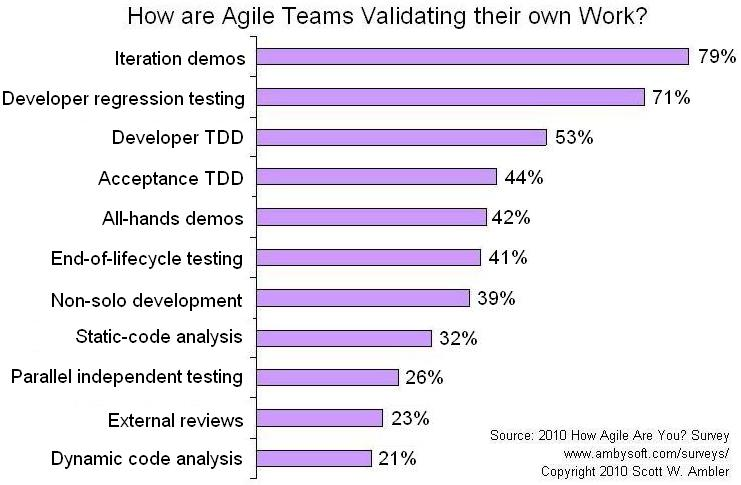
\includegraphics[scale=.4]{agileCriteria2010Validating}
    \caption{Como times ágeis validam seu próprio trabalho?}
    \label{fig:wambler-agile-2010}
  \end{minipage}
  \hspace{0.5cm}
  \begin{minipage}[b]{0.45\linewidth}
    \centering
    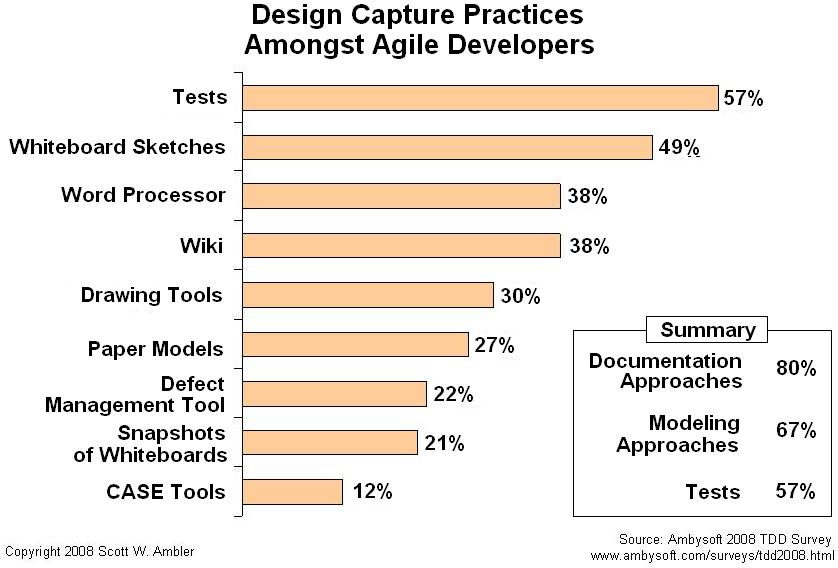
\includegraphics[scale=.35]{tddDesignPractices}
    \caption{Maneiras de captura de design entre desenvolvedores ágeis}  
    \label{fig:wambler-tdd-2008}
  \end{minipage}
\end{figure}			

%% ------------------------------------------------------------------------- %%
\section{Contribuições}

Este trabalho não tenta inferir uma possível relação de causa entre TDD e
bom design, mas sim entender como a prática influencia as decisões de 
design tomadas por um programador praticante de TDD.

O objetivo desta pesquisa é entender como TDD influencia essas decisões sob vários
pontos de vista diferentes, como acoplamento, coesão e simplicidade. 
A análise será feita por meio de dados que serão
capturados baseados na percepção de programadores que realizam a prática no seu
dia-a-dia de trabalho.
Os objetivo principal da pesquisa é \textbf{entender a influência de TDD no
design de sistemas orientados a objetos}.

Para compreender a influência, essa pesquisa tenta responder às questões listadas
abaixo:

\begin{enumerate}

  \item Como o teste guia o desenvolvedor durante a atividade de
  design?

  \item Como a prática de TDD influencia o programador no processo de 
  design de classes, do ponto de vista do acoplamento?

  \item Como a prática de TDD influencia o programador no processo de 
  design de classes, do ponto de vista do coesão?

  \item Como a prática de TDD influencia o programador no processo de 
  design de classes, do ponto de vista da simplicidade?

\end{enumerate}

%% ------------------------------------------------------------------------- %%
\section{Organização do trabalho}

Este trabalho está dividido da seguinte maneira: 

\begin{itemize}
	\item O Capítulo \ref{cap:tdd} discute sobre a prática de TDD, com ênfase no
	ponto de vista do design.
  
	\item O Capítulo \ref{cap:trabalhos-relacionados} mostra trabalhos já
	realizados pela academia sobre os efeitos de TDD.

 	\item O Capítulo \ref{cap:qualitativo} discute métodos qualitativos de
 	pesquisa e suas características;

	\item O Capítulo \ref{cap:planejamento} discute o planejamento do experimento,
	bem como o processo de captura de dados e análise;

	\item O Capítulo \ref{cap:discussao} apresenta os resultados encontrados e
	discute em cima dos mesmos.
	
	\item O Capítulo \ref{cap:ameacas} discute as possíveis ameaças dos resultados
	encontrados na pesquisa.
	
	\item O Capítulo \ref{cap:conclusoes} resume o trabalho realizado a apresenta
	possibilidades de trabalhos futuros.
\end{itemize}

